\subsubsection{Contexts Facilitating Adult Development and Aging}

%insert

\subsubsection{Physical and Motor Fitness as Facilitators of Cognitive and Emotional Plasticity }

%insert

\subsubsection{Developmental Regulation and Self-Regulation as Facilitators of Adult Development and Aging}

%insert

\subsubsection{Two Types of Positive Personality Development: Adjustment and Growth }

\paragraph{}
\begin{flushleft}
\textbf{Research Program}
\end{flushleft}

Does personality stay stable after young adulthood or is there continued change throughout middle and later adulthood? For decades, this question has caused heated debate. In recent years, a consensus has emerged based on contemporary cross-cultural as well as longitudinal evidence. This consensus confirms that indeed there is personality change in middle and later adulthood. Many authors have labeled this change, personality maturation or growth. In somewhat simplified terms the observed pattern is as follows: Neuroticism declines, conscientiousness and agreeableness increase. At the same time it has been argued that this pattern of personality change is the result of coping with the developmental tasks of adulthood and thus increased adjustment. In this research area, we are interested in exploring the different ways of operationalizing adjustment and growth, and also finding out about their developmental dynamics. 

\paragraph{}
\begin{flushleft}
\textbf{Research Highlihts 2007/2008}
\end{flushleft}

Our two goals were to develop and validate a performance measure of personal wisdom (PW), and to examine age differences. Based on the Berlin wisdom paradigm and growth theories of personality, five criteria of PW were developed. A sample of 83 younger (20-40) and 78 older adults (60-80) thought aloud about a PW task. Transcribed answers were rated. Validity was established with regard to indicators of personality growth, subjective well-being, intelligence, critical life events, as well as general wisdom (GW; see Fig. 14). As expected, no age differences were obtained on the basic criteria and negative age differences were found on the meta-criteria indexing PW. Fluid intelligence and openness to new experience partially mediated these differences. It is argued that on average and for current cohorts, age-related changes in psychological functioning may act as hindrances to PW.

\begin{figure}[htb]
  \begin{center}
    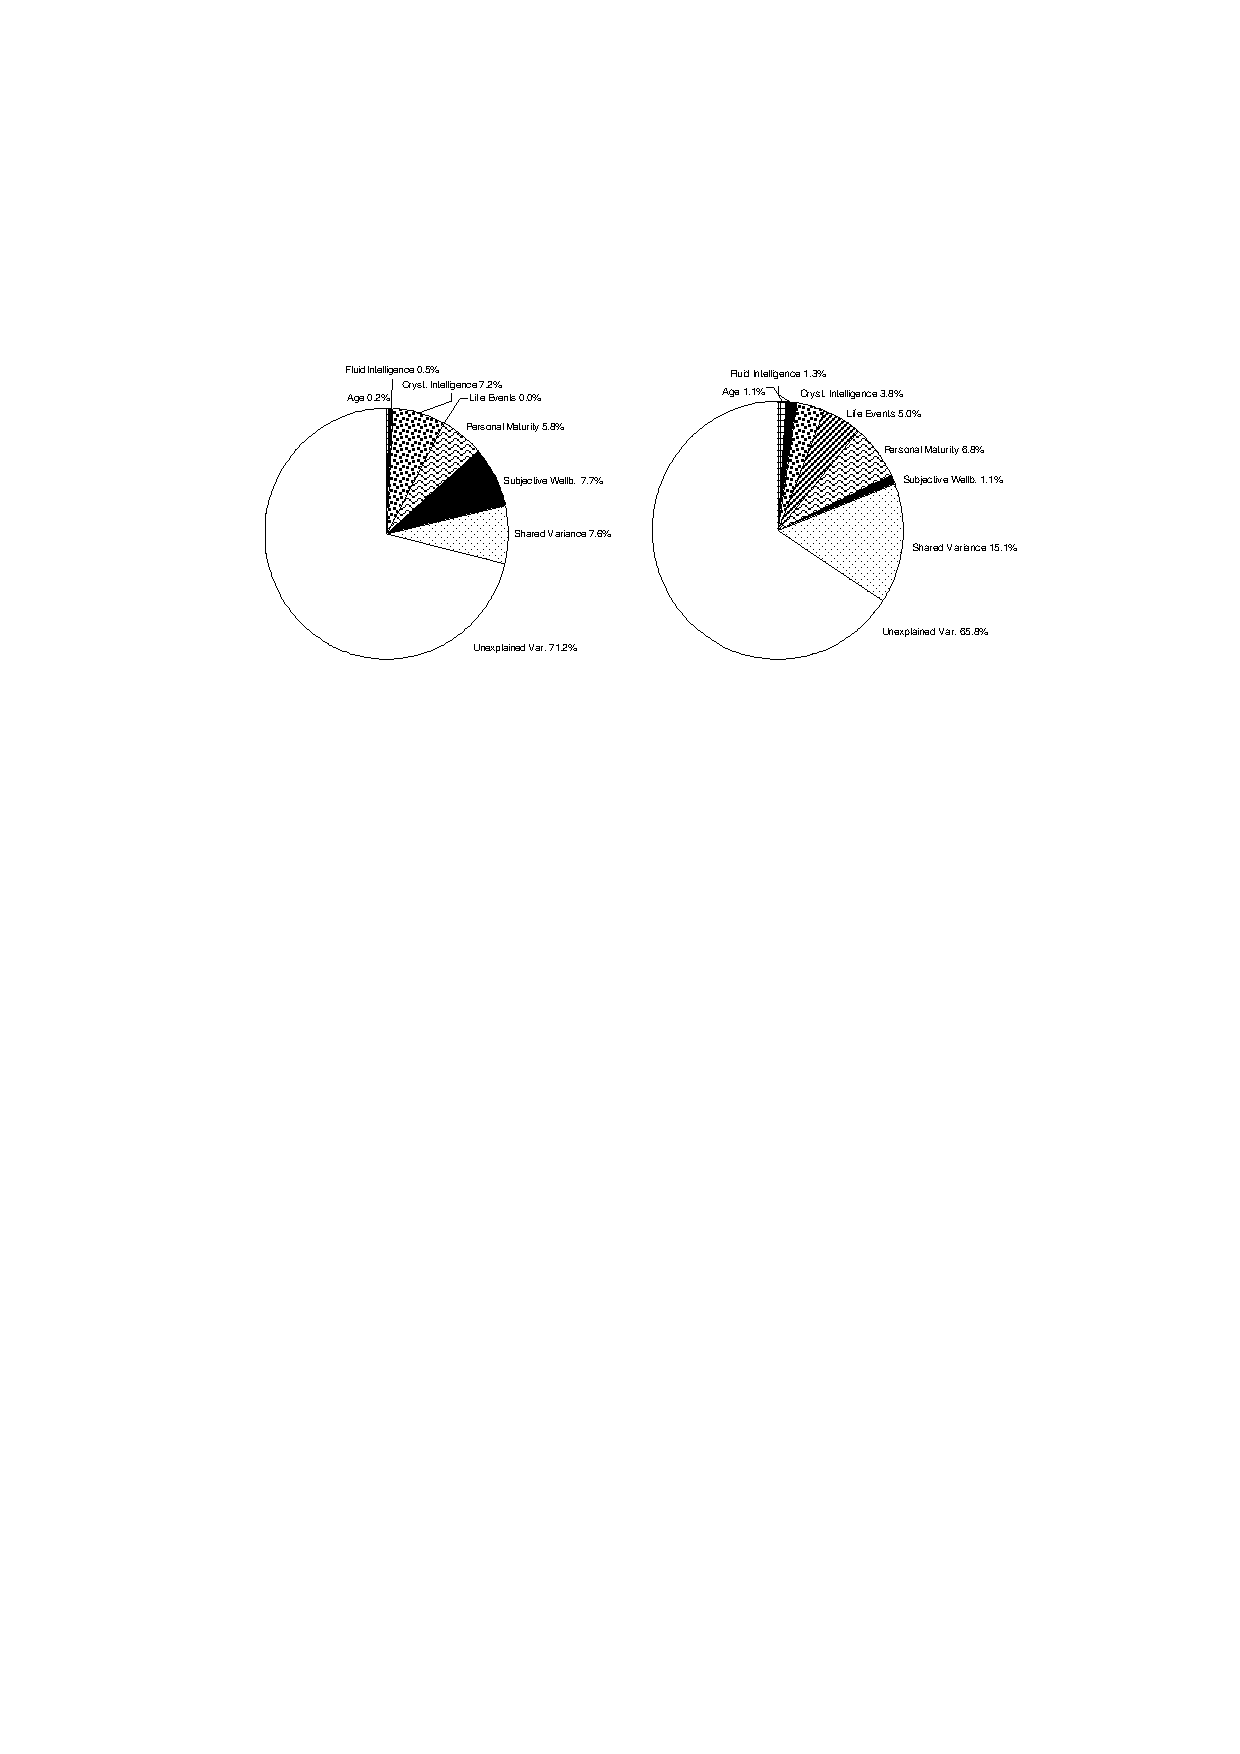
\includegraphics[width=0.5\textwidth,height=5.5cm]{fig14.pdf}
    \caption{Predictive validity of two wisdom measures (results of commonality analysis; Mickler \& Staudinger, 2008)}
  \end{center}
\end{figure}

\subsubsection{Collaborations}

\begin{itemize}

\item Brandeis University; Prof. Margie Lachman, PhD
\item Humboldt University, Berlin�; Dr. Charlotte Mickler
\item Jacobs University, JCLL�; Prof. Dr. Ben Godde
\item Jacobs University, JCLL�; Prof. Dr. Klaus Sch�mann
\item Jacobs University, JCLL�; Dr. Claudia Voelcker-Rehage
\item Max Planck Institute for Human Development, Berlin; Prof. Dr. Ulman Lindenberger  
\item Stanford University; Prof. Laura Carstensen, PhD
\item University of Florida, Gainsville, FLA; Prof. Manfred Diehl, PhD
\item University of Frankfurt; Prof. Dr. Tilmann Habermas
\item University of Klagenfurt;Prof. Dr. Judith Gl�ck
\item University of Heidelberg�; Prof. Dr. Hans-Werner Wahl
\item University of Hildesheim; Prof. Dr. Werner Greve
\item University of Michigan�; Prof. Patricia Reuter-Lorenz, PhD
\end{itemize}

\subsubsection{Other Professional Activities}

\begin{itemize}

\item Alexander von Humboldt Stiftung, Member of Selection Committee
\item Berlin-Institut f�r Bev�lkerung und Entwicklung, Member of the Advisory Board 
\item German Center for Gerontology, DZA, Member of the Scientific Board
\item German Psychological Society, President
\item Joint Academy Network "Aging in Germany" (Leopoldina, acatech), Co-Speaker
\item Leopoldina National Academy of Sciences, Vice President
\item Margret M. and Paul B. Baltes Foundation, Chair 
\item Max Planck International Research Network on Aging (MAXNET Aging), Senior Fellow 

\end{itemize}

